\documentclass[11pt]{article}
\usepackage[margin=1in]{geometry}
\usepackage{amsmath,amssymb}
\usepackage{tikz}
\usetikzlibrary{positioning,arrows.meta,calc}
\usepackage{booktabs}
\usepackage{caption}

% ---- namespaced styles (p2) ----
\tikzset{
  p2ent/.style={circle, draw=black!65, line width=0.7pt, minimum size=9.5mm,
                inner sep=0pt, font=\small\bfseries},
  p2lab/.style={font=\scriptsize},
  p2rel/.style={draw=black!65, line width=0.7pt},
  p2edgelab/.style={font=\scriptsize, fill=white, inner sep=1.5pt},
}
\newcommand{\pTwoTypeA}{blue!12}   % author / user
\newcommand{\pTwoTypeP}{orange!20} % paper / movie / business (target type)
\newcommand{\pTwoTypeX}{green!14}  % attribute types
\newcommand{\pTwoTypeY}{purple!12} % venue / institution

\begin{document}

\section*{Schema drafts}

\subsection*{DBLP}
\begin{center}
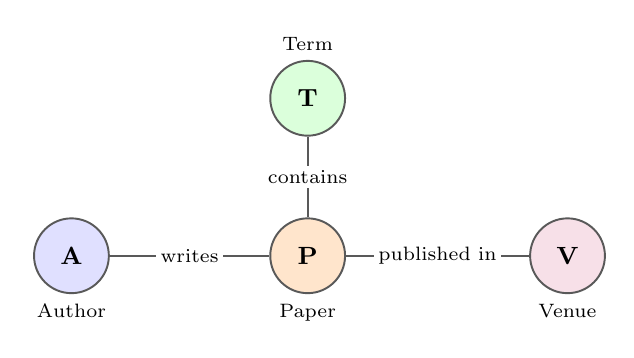
\begin{tikzpicture}[scale=1.0]
  \node[p2ent, fill=\pTwoTypeP, label={[p2lab]below:Paper}] (P) at (0,0) {P};
  \node[p2ent, fill=\pTwoTypeA, label={[p2lab]below:Author}] (A) at (-3.0,0) {A};
  \node[p2ent, fill=\pTwoTypeY, label={[p2lab]below:Venue}] (V) at (3.3,0) {V};
  \node[p2ent, fill=\pTwoTypeX, label={[p2lab]above:Term}] (T) at (0,2.0) {T};
  \draw[p2rel] (A) -- node[p2edgelab]{writes} (P);
  \draw[p2rel] (P) -- node[p2edgelab]{published in} (V);
  \draw[p2rel] (P) -- node[p2edgelab]{contains} (T);
\end{tikzpicture}
\end{center}

\subsection*{ACM}
\begin{center}
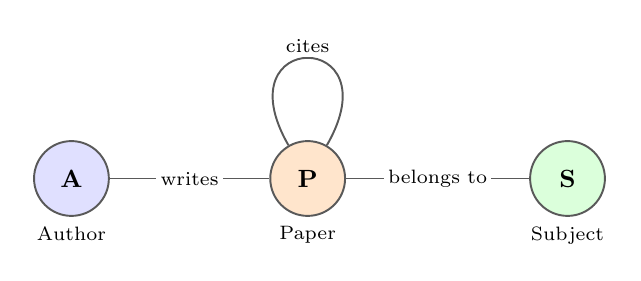
\begin{tikzpicture}
  \node[p2ent, fill=\pTwoTypeP, label={[p2lab]below:Paper}] (P) at (0,0) {P};
  \node[p2ent, fill=\pTwoTypeA, label={[p2lab]below:Author}] (A) at (-3.0,0) {A};
  \node[p2ent, fill=\pTwoTypeX, label={[p2lab]below:Subject}] (S) at (3.3,0) {S};
  \draw[p2rel] (A) -- node[p2edgelab]{writes} (P);
  \draw[p2rel] (P) -- node[p2edgelab]{belongs to} (S);
  \draw[p2rel] (P) to[out=60,in=120,looseness=9] node[p2edgelab,above]{cites} (P);
\end{tikzpicture}
\end{center}

\subsection*{IMDB}
\begin{center}
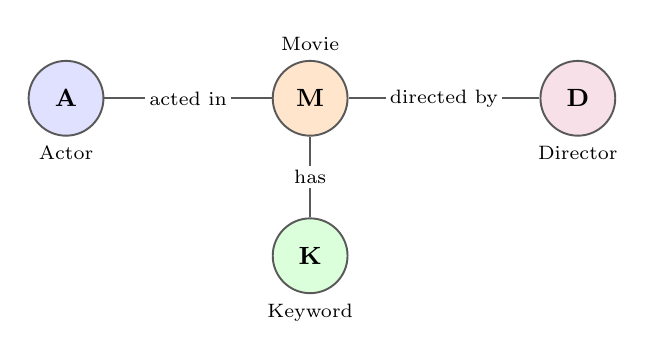
\begin{tikzpicture}
  \node[p2ent, fill=\pTwoTypeP, label={[p2lab]above:Movie}] (M) at (0,0) {M};
  \node[p2ent, fill=\pTwoTypeA, label={[p2lab]below:Actor}] (A) at (-3.1,0) {A};
  \node[p2ent, fill=\pTwoTypeY, label={[p2lab]below:Director}] (D) at (3.4,0) {D};
  \node[p2ent, fill=\pTwoTypeX, label={[p2lab]below:Keyword}] (K) at (0,-2.0) {K};
  \draw[p2rel] (M) -- node[p2edgelab]{acted in} (A);
  \draw[p2rel] (M) -- node[p2edgelab]{directed by} (D);
  \draw[p2rel] (M) -- node[p2edgelab]{has} (K);
\end{tikzpicture}
\end{center}

\subsection*{ogbn-mag}
\begin{center}
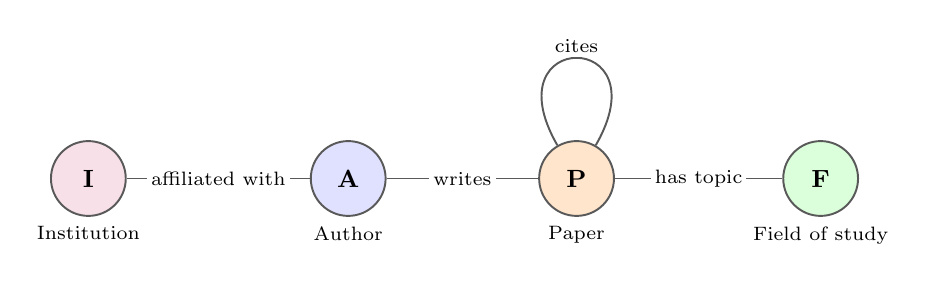
\begin{tikzpicture}
  \node[p2ent, fill=\pTwoTypeY, label={[p2lab]below:Institution}] (I) at (-6.2,0) {I};
  \node[p2ent, fill=\pTwoTypeA, label={[p2lab]below:Author}] (A) at (-2.9,0) {A};
  \node[p2ent, fill=\pTwoTypeP, label={[p2lab]below:Paper}] (P) at (0,0) {P};
  \node[p2ent, fill=\pTwoTypeX, label={[p2lab]below:{Field of study}}] (F) at (3.1,0) {F};
  \draw[p2rel] (A) -- node[p2edgelab]{affiliated with} (I);
  \draw[p2rel] (A) -- node[p2edgelab]{writes} (P);
  \draw[p2rel] (P) -- node[p2edgelab]{has topic} (F);
  \draw[p2rel] (P) to[out=60,in=120,looseness=9] node[p2edgelab,above]{cites} (P);
\end{tikzpicture}
\end{center}

\subsection*{LastFM}
\begin{center}
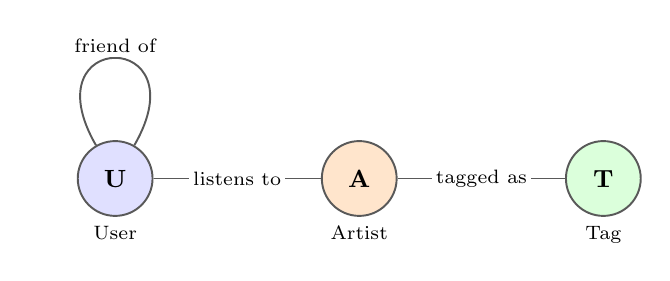
\begin{tikzpicture}
  \node[p2ent, fill=\pTwoTypeA, label={[p2lab]below:User}] (U) at (-3.1,0) {U};
  \node[p2ent, fill=\pTwoTypeP, label={[p2lab]below:Artist}] (A) at (0,0) {A};
  \node[p2ent, fill=\pTwoTypeX, label={[p2lab]below:Tag}] (T) at (3.1,0) {T};
  \draw[p2rel] (U) -- node[p2edgelab]{listens to} (A);
  \draw[p2rel] (A) -- node[p2edgelab]{tagged as} (T);
  \draw[p2rel] (U) to[out=60,in=120,looseness=9] node[p2edgelab,above]{friend of} (U);
\end{tikzpicture}
\end{center}

\subsection*{Yelp}
\begin{center}
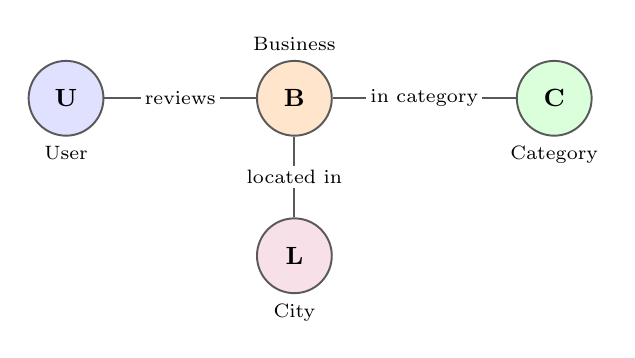
\begin{tikzpicture}
  \node[p2ent, fill=\pTwoTypeP, label={[p2lab]above:Business}] (B) at (0,0) {B};
  \node[p2ent, fill=\pTwoTypeA, label={[p2lab]below:User}] (U) at (-2.9,0) {U};
  \node[p2ent, fill=\pTwoTypeX, label={[p2lab]below:Category}] (C) at (3.3,0) {C};
  \node[p2ent, fill=\pTwoTypeY, label={[p2lab]below:City}] (L) at (0,-2.0) {L};
  \draw[p2rel] (U) -- node[p2edgelab]{reviews} (B);
  \draw[p2rel] (B) -- node[p2edgelab]{in category} (C);
  \draw[p2rel] (B) -- node[p2edgelab]{located in} (L);
\end{tikzpicture}
\end{center}

\end{document}
